\chapter{Processor Core}

Chapter \ref{chp:system-overview} describes how vector graphics are supported and integrated into the \vthreek architecture.
This chapter elaborates on how the processor core is designed, focusing especially on features directly related to vector graphics.

\section{The \vthreek processor}

The processor core is the main processing and control unit in the \vthreek architecture.
As depicted in Figure \ref{fig:system-overview}, the processor core reads instructions from the instruction memory, and writes/reads data to/from the data and scene memories.
The processor core is designed as a multi-cycle, MIPS-inspired processor with features added to support processing of vector graphics.
When planning which features to include and which techniques to utilize, the group considered features like pipelining and even multicore designs to improve performance.
In the end, the decision was made to make the initial design simple, but keep efficiency and performance in mind.

\begin{figure}[H]
    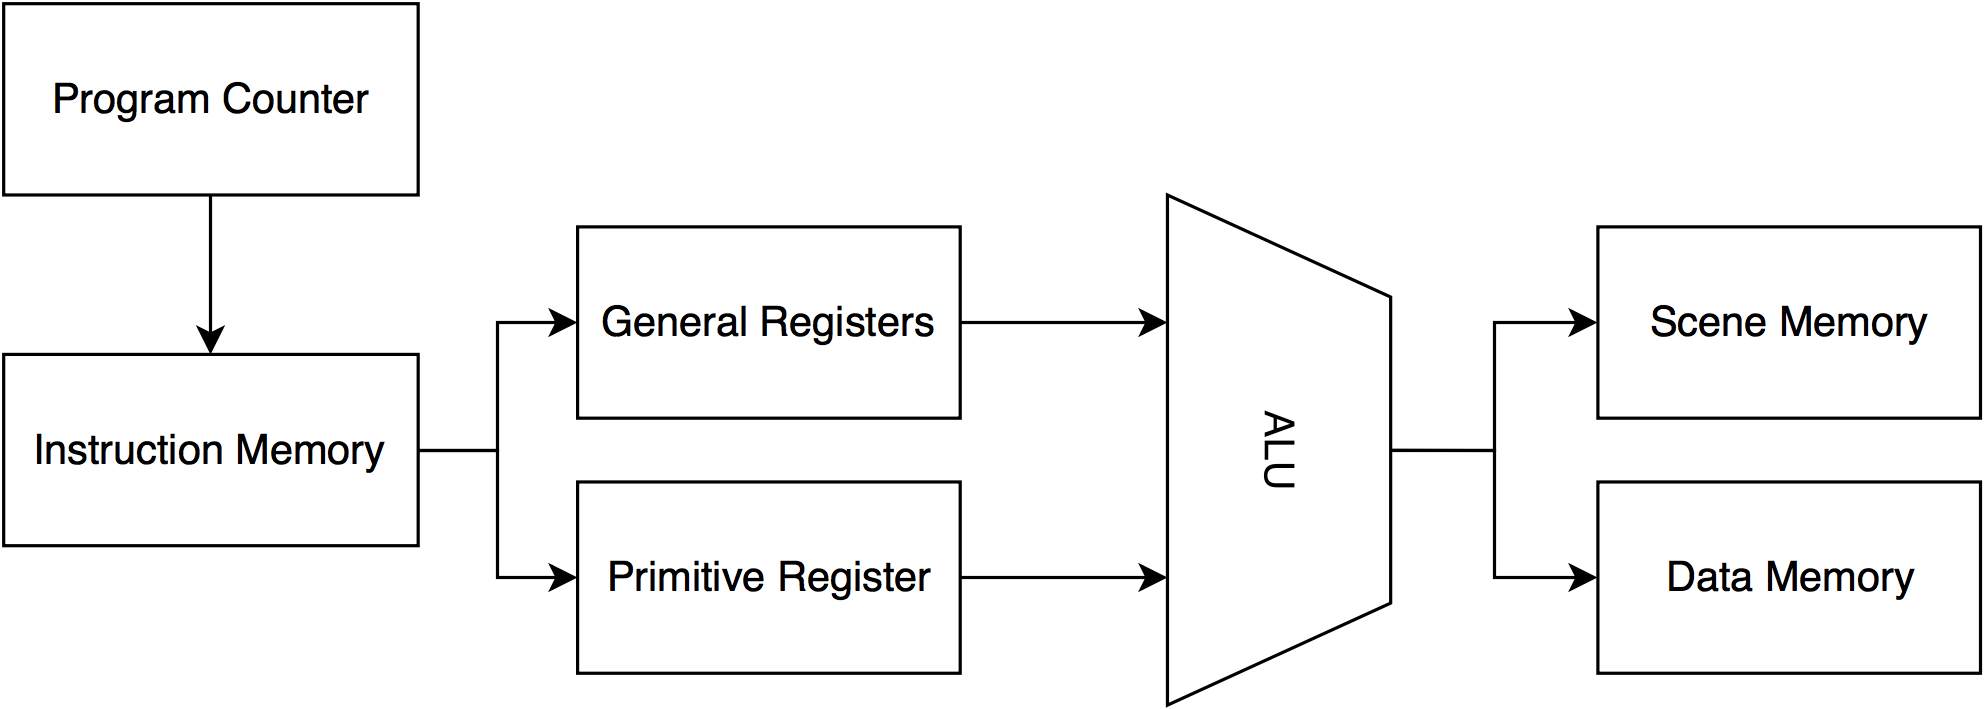
\includegraphics[width=\linewidth]{images/core-components.png}
    \caption{Overview of the main components in the processor core.}
    \label{fig:core-components}
\end{figure}

Figure \ref{fig:core-components} shows how data flows through the subcomponents of the processor core.
In addition to the components in the figure, the core includes a control unit.
Each component is described in detail in their respective section below, the following is a short introduction to their responsibilities.

\begin{description}
    \item[Program counter] \hfill \\
        The program counter keeps track of the address of the next instruction to be executed.
        Depending on the instruction currently being executed, the program counter is either incremented or overwritten.
    \item[Control] \hfill \\
        The control unit keeps track of the state of the processor, namely fetch, execute and stall, and issues the appropriate control signals to the other components.
    \item[Register] \hfill \\
        The register bank is the short term memory of the core, feeding operands to the ALU, and recieving data which may be stored based on the control signals.
    \item[ALU] \hfill \\
        The ALU performs operations on the data it receives from the register unit and outputs the result.
    \item[Primitive Register] \hfill \\
        The primitive register is a special purpose register, containing the vector primitive that the core is currently processing.
\end{description}

\section{Instruction Format}

Instructions in the \vthreek architecture are 32 bits wide.
As opposed to the MIPS architecture, they can't all be grouped into categories based on their format.
They do however share some common traits.
All instructions start with a 6-bit opcode, a unique identifier for each instruction.
The remaining bits are used either to address registers, to encode immediate values or as a combination.
Some instructions also have don't care bits, parts of the instruction that can be either 1 or 0 without influencing the outcome of execution.
For instructions that address one or more registers, a general convention of using the five bits directly after the opcode for the destination register and addressing source registers in successive five bit chunks.
Figure \ref{fig:instruction-format} shows how various parts of an instruction word is utilized.

\begin{figure}[h!]
    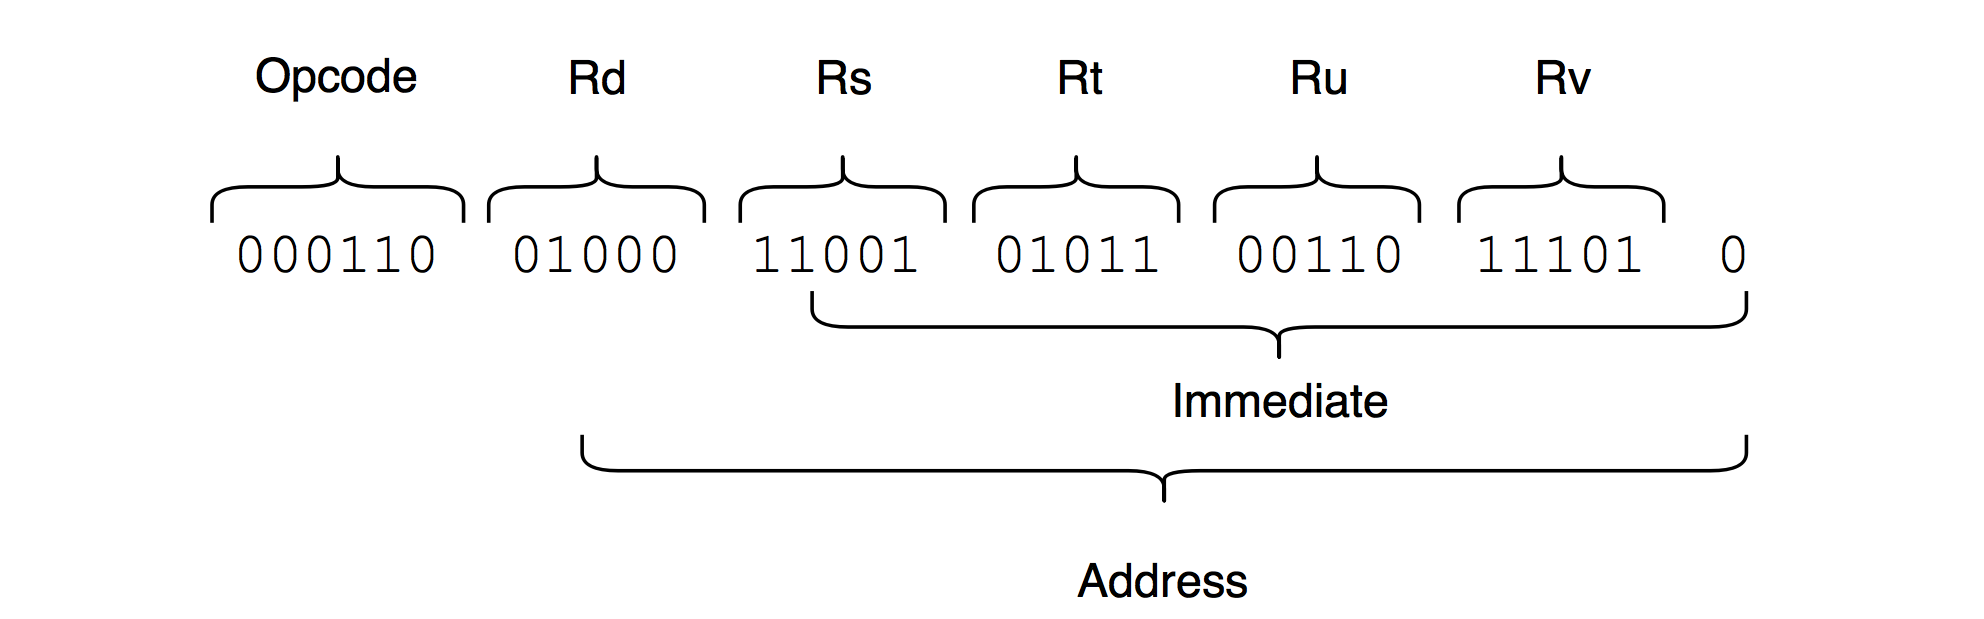
\includegraphics[width=\linewidth]{images/instruction-format.png}
    \caption{\vthreek instruction format.}
    \label{fig:instruction-format}
\end{figure}

As an example, the \texttt{jmp} instruction is encoded with the opcode \texttt{000001}, seven don't care bits followed by the 19-bit jump target.
The \texttt{bezcube} instruction initializes a cubic Bézier primitive into the primitive register, reading the coordinates of the four control points from four general purpose registers.
With 32 general purpose registers, five bits are needed to address them.
That means that the \texttt{bezcube} instruction is encoded with its six bit opcode, \texttt{000111}, followed by five don't care bits, then four 5-bit chunks, one for each register.
The final bit is also don't care.

\section{Data Path}

\begin{figure}[h!]
    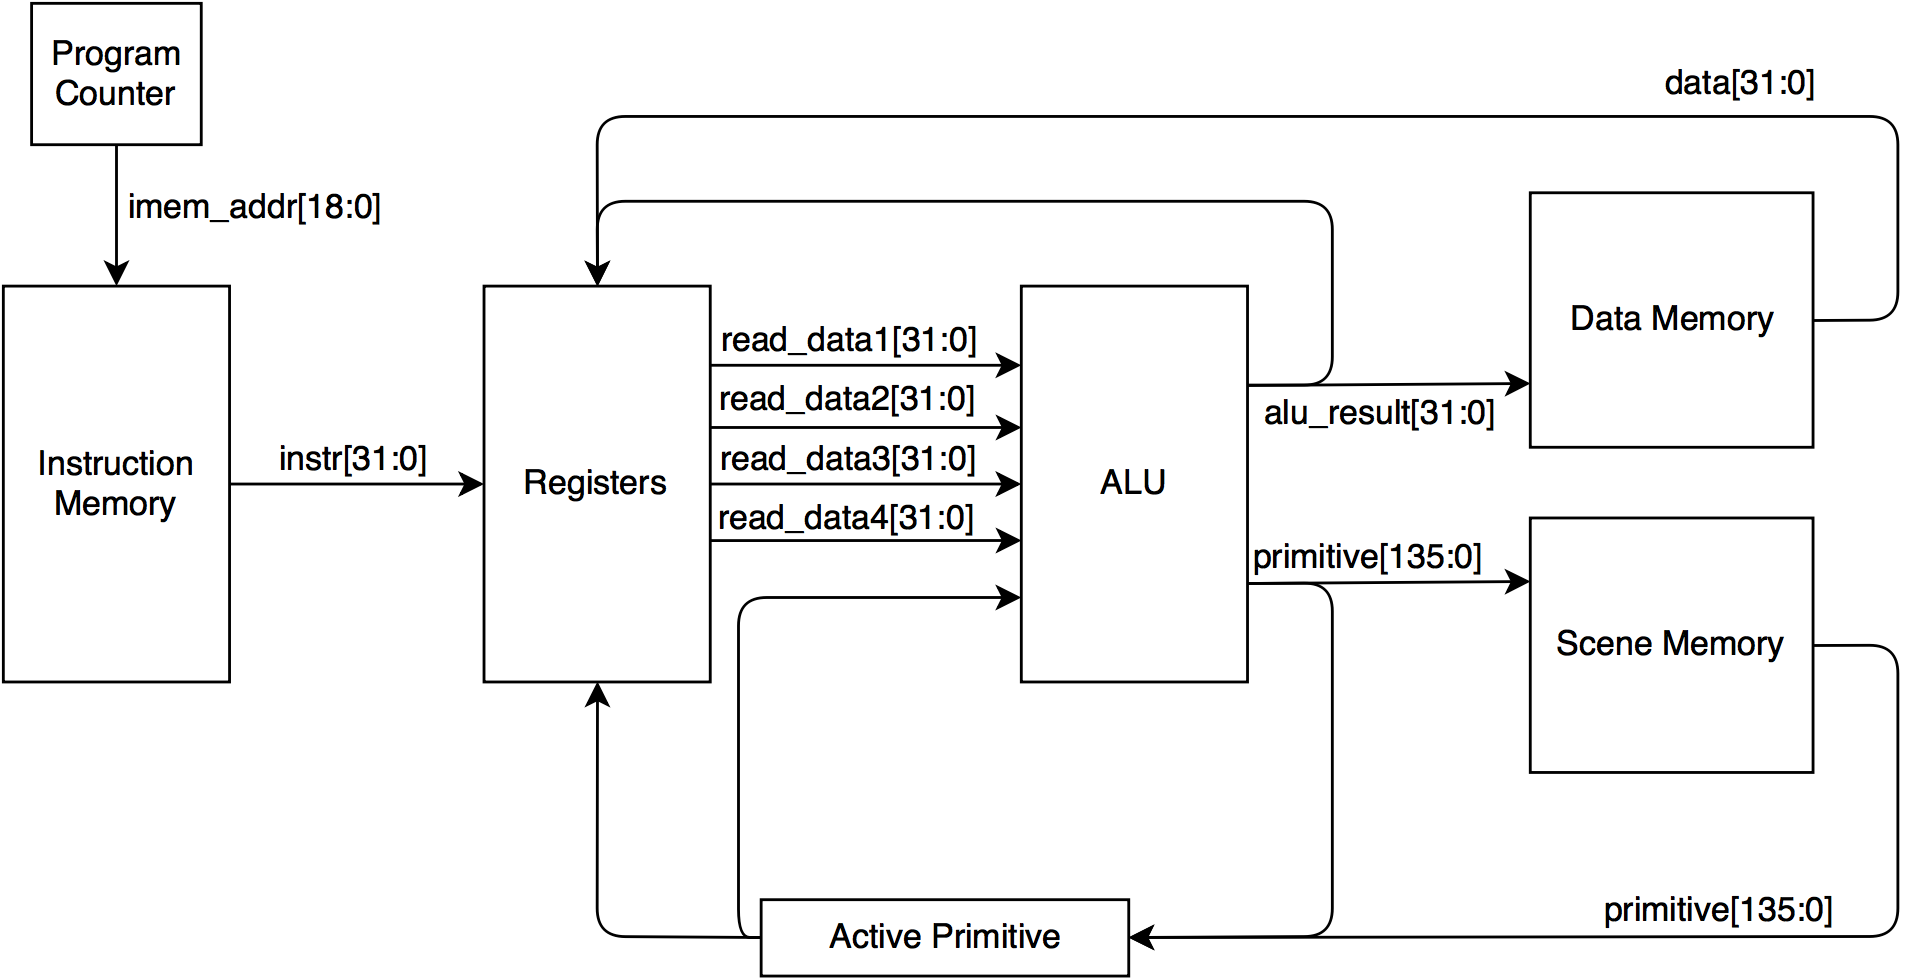
\includegraphics[width=\linewidth]{images/Data_path.png}
    \caption{RTL sketch of the data path.}
    \label{fig:datapath}
\end{figure}

The data path of the \vthreek architecture consists of a registerfile encapsulating the 32 general purpose registers, a separate, special purpose, 136-bit vector primitive register, a functional unit, the ALU, and instruction, scene and data memories.
To explain how these work together, each component will be explained in the order with which an instruction being executed interacts with them.

\subsection{Instruction Memory}

\begin{figure}[h!]
    \centering
    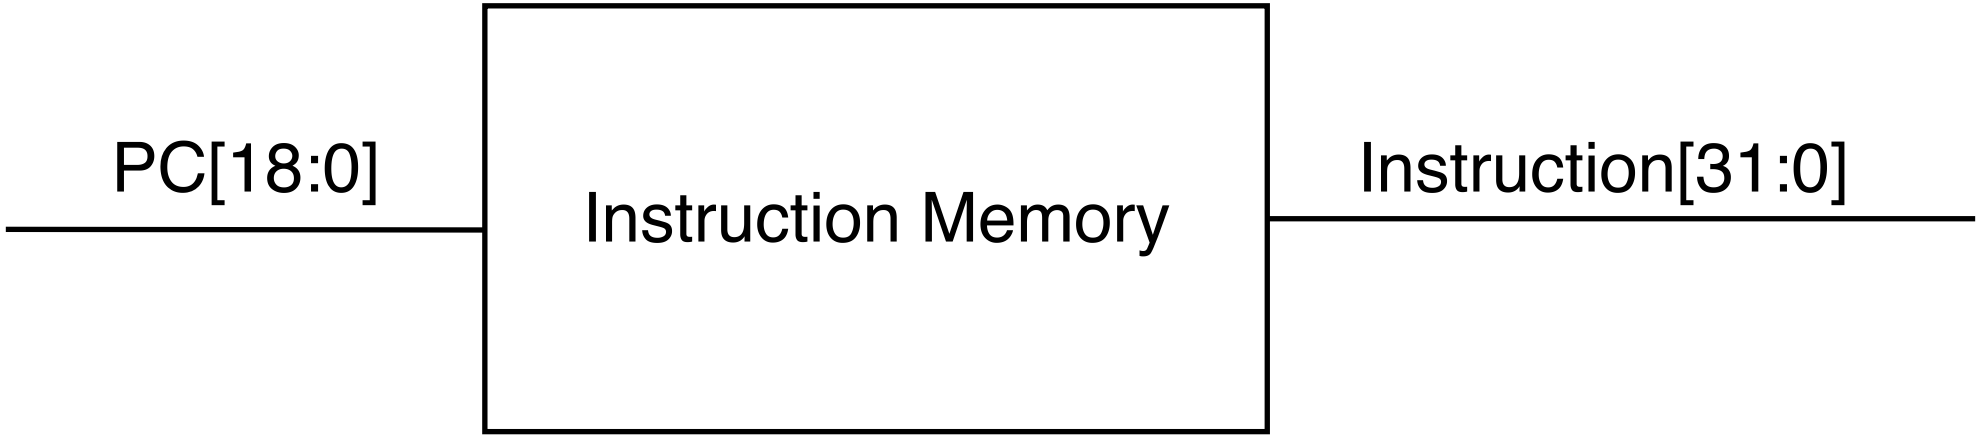
\includegraphics[width=0.6\linewidth]{images/instruction-memory.png}
    \caption{I/O for the instruction memory.}
    \label{fig:instruction-memory}
\end{figure}

Figure \ref{fig:instruction-memory} shows the signals going into and coming out of the instruction memory.
The program counter value is the address of the desired instruction.
Due to only being able to read 16 bits at a time from the SRAM, the group implemented a stateful instruction fetch module encapsulating the instruction memory.

\subsection{Registers}

\begin{figure}[h!]
    \centering
    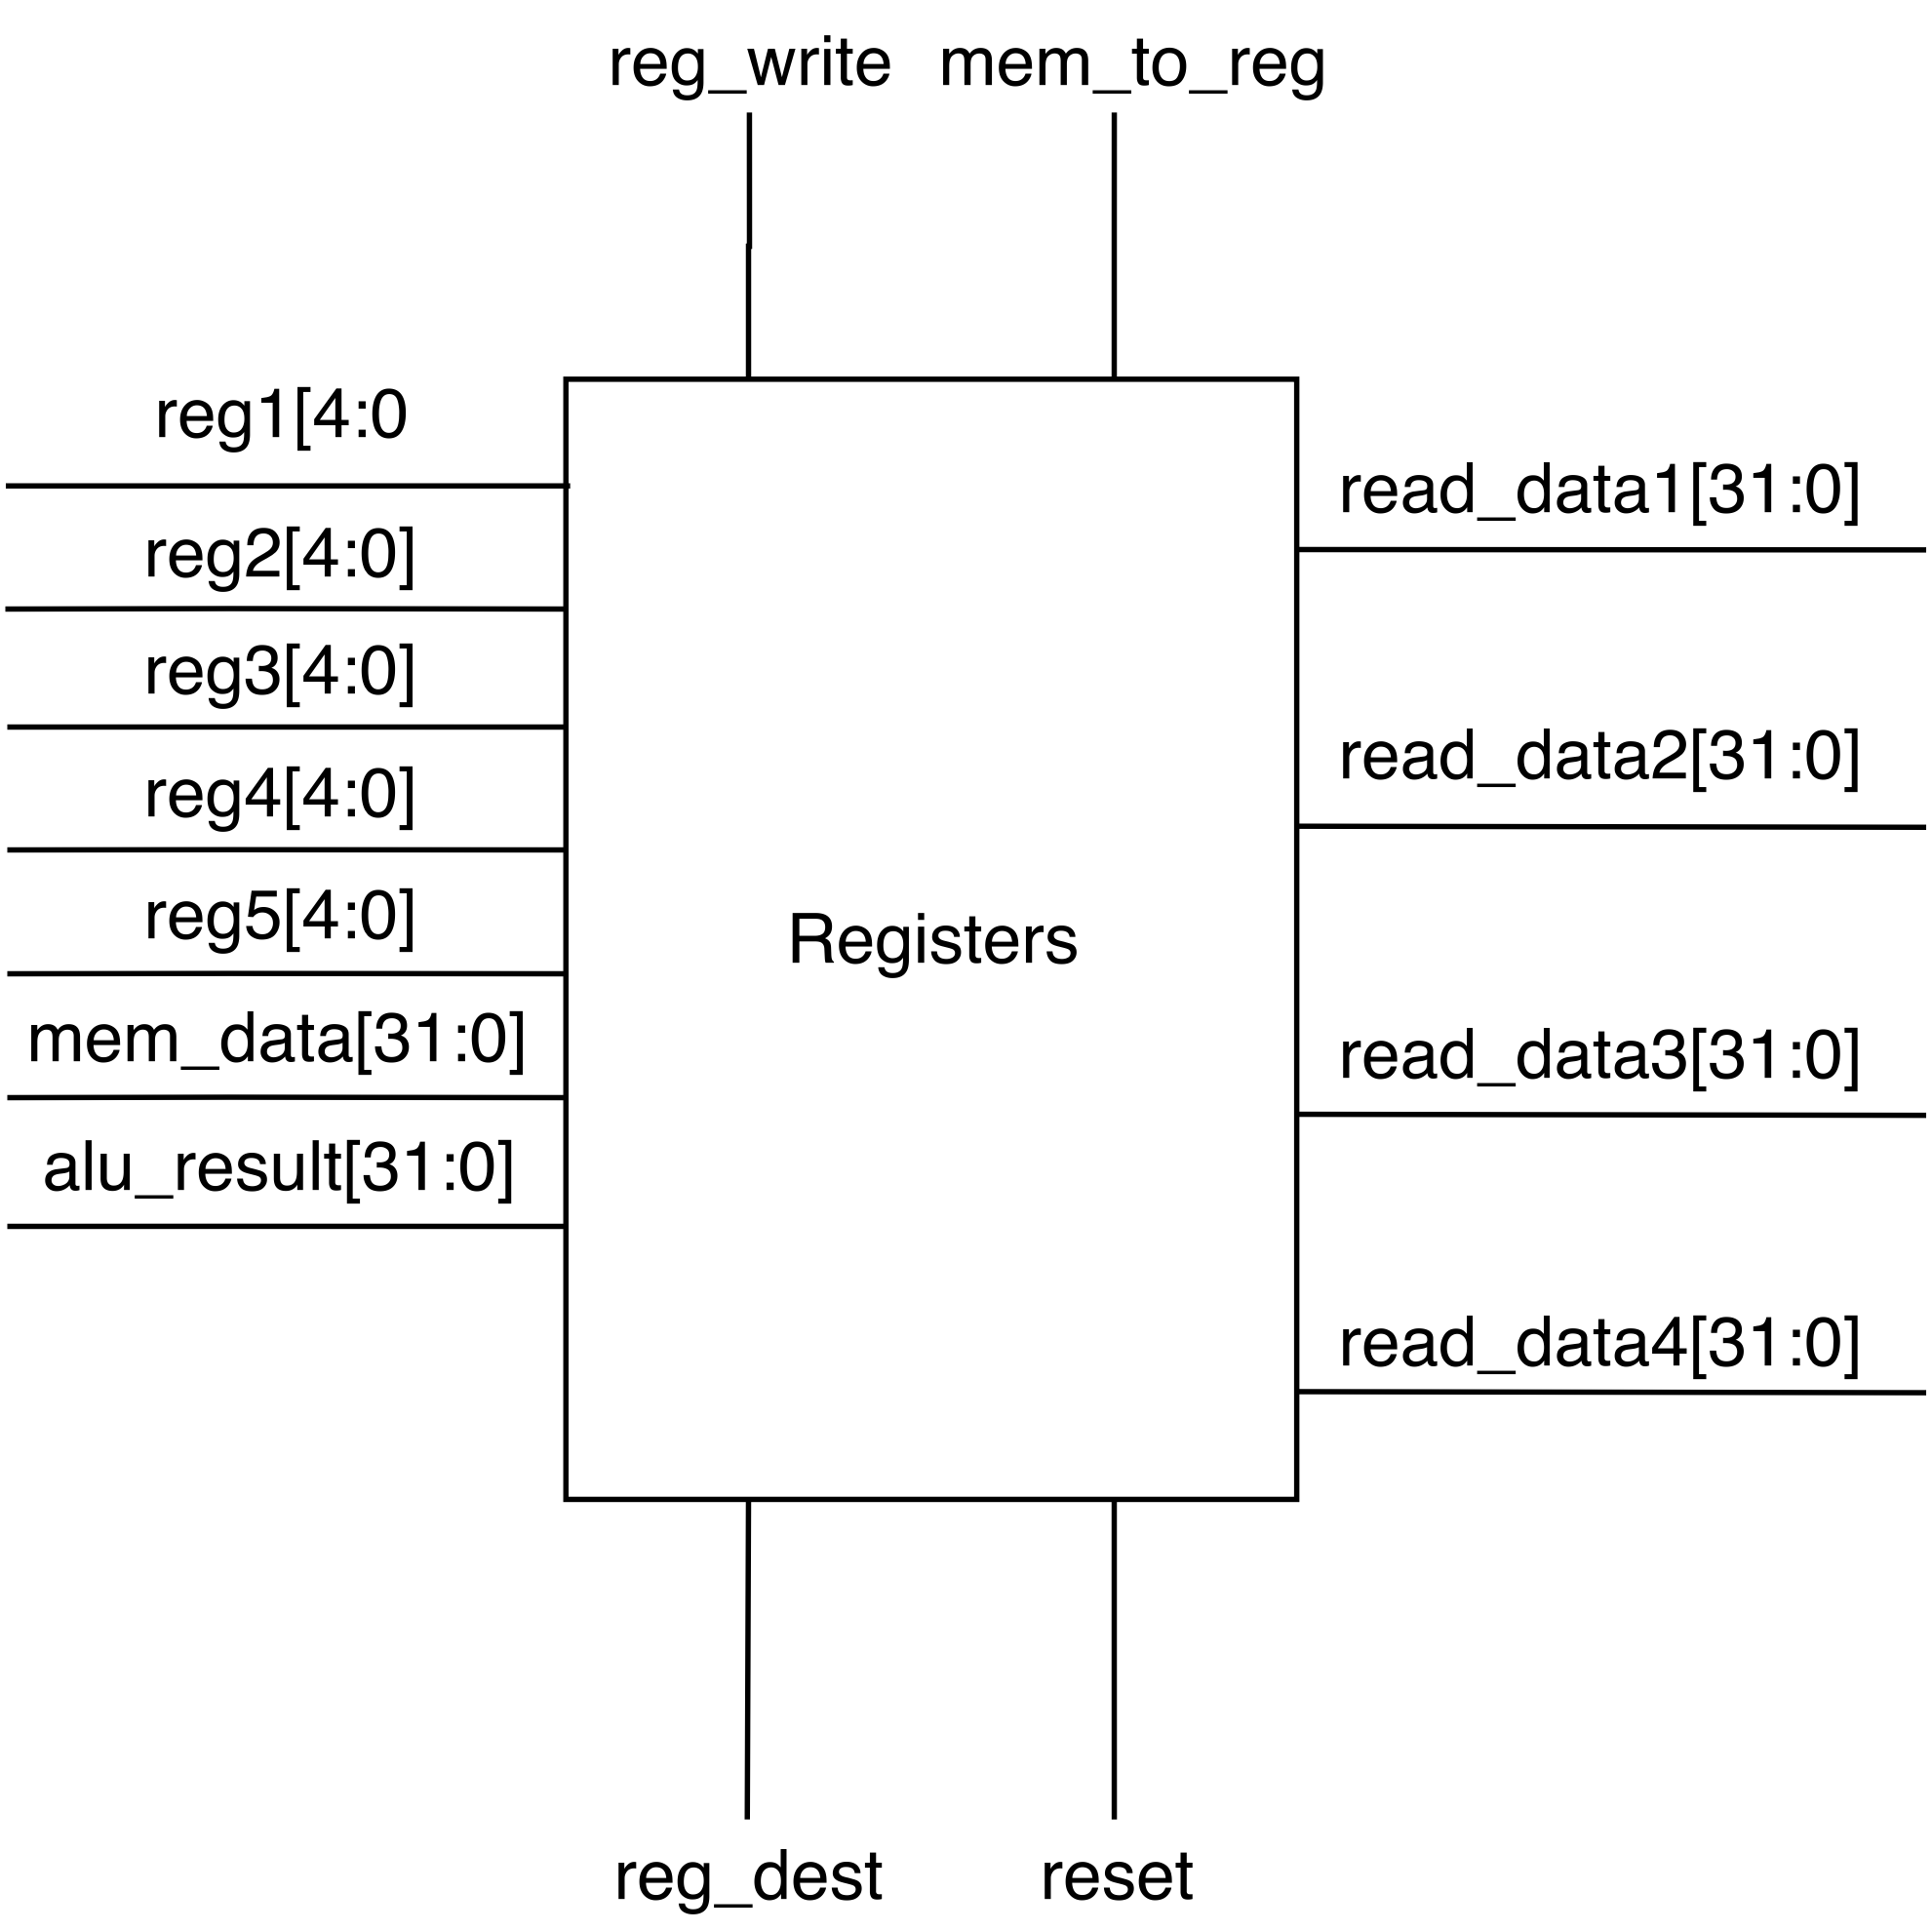
\includegraphics[width=0.6\linewidth]{images/registers.png}
    \caption{I/O for the register module.}
    \label{fig:registers}
\end{figure}

After being read from the instruction memory, an instruction is decoded and wired as input to the register module.

The \vthreek architecture provides 32 32-bit general purpose registers.
These are organised into a registerfile.
As can be seen in Figure \ref{fig:registers}, this module receives five register addresses.
The values in the addressed registers are continuously output on the \texttt{read\_data} signals.
32-bit input values are taken as input from the ALU and the data memory, to potentially be written to into a register.
There are four control signals, \texttt{reset, mem\_to\_reg, reg\_dest} and \texttt{reg\_write}.
\texttt{reset} signals the module to clear all registers of their contents.
\texttt{reg\_write} signals wether or not data should be written in the current cycle.
\texttt{reg\_dest} indicates which of the \texttt{regX} registers should be used as the destination register.
Similarily, \texttt{mem\_to\_reg} indicates wether the data from memory or the alu result should be written.

The special purpose primitive register functions in much the same way, only with a single register.
Its inputs, outputs and control signals can be seen in Figure \ref{fig:primitive-register}.
Since there is only one register to address, the primitive register doesn't take any part of the instruction as input, but rather outputs its current value continuously.
Control signals only determine wether or not the register contents should be overwritten and if yes, what data source should be used to overwrite.

\begin{figure}[h!]
    \centering
    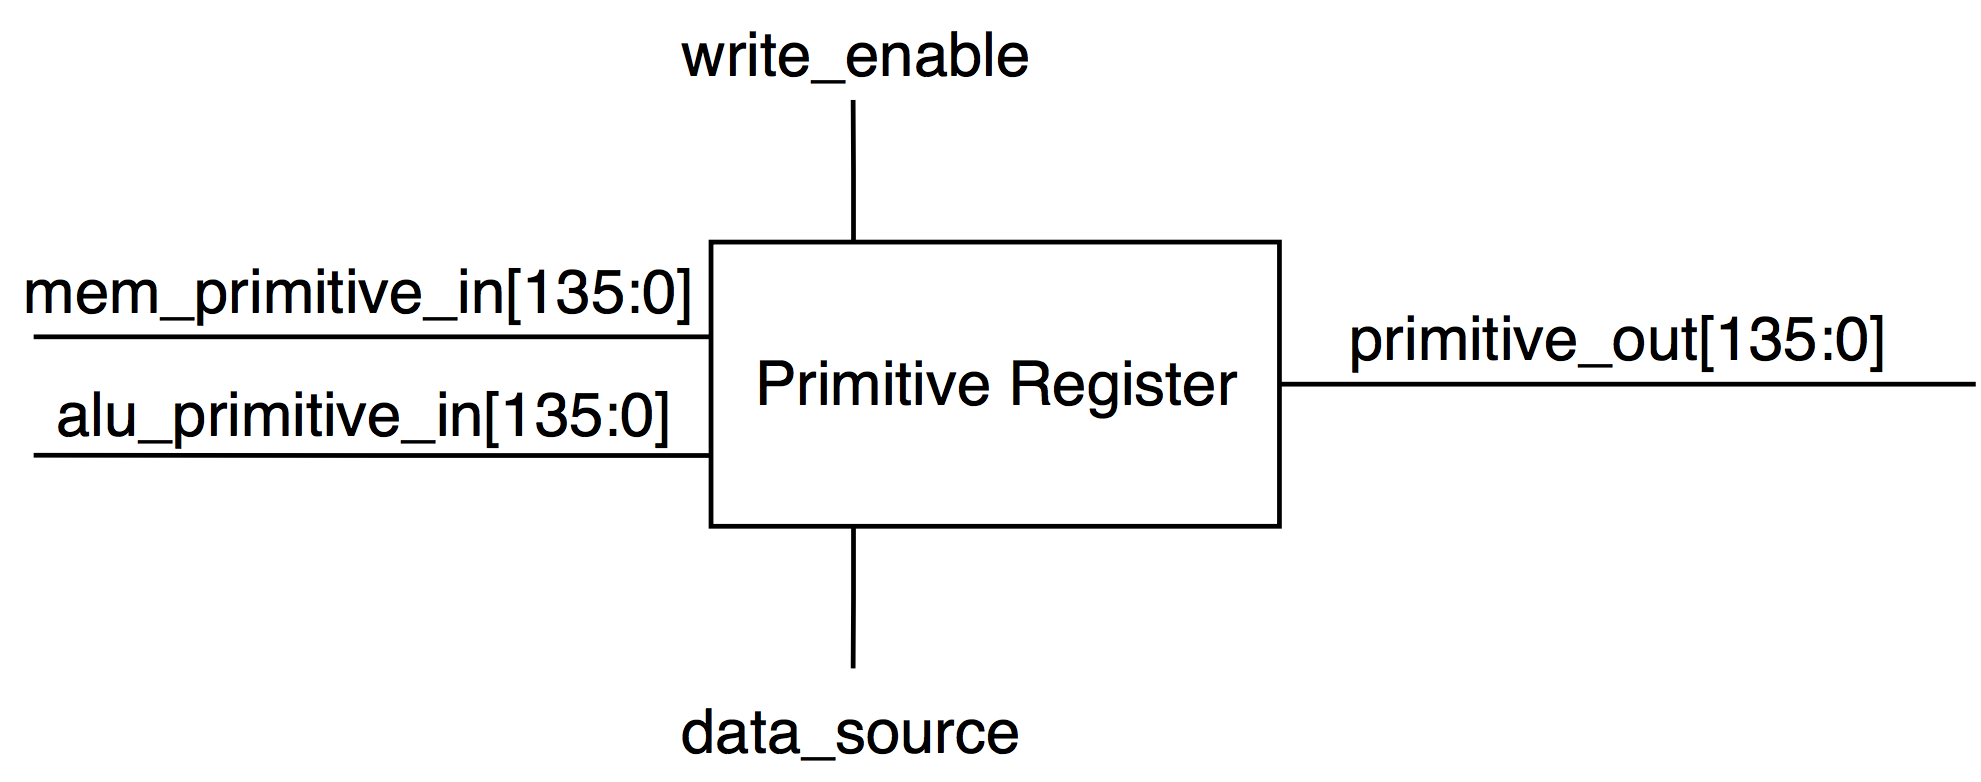
\includegraphics[width=0.6\linewidth]{images/primitive-register.png}
    \caption{I/O for the primitive register.}
    \label{fig:primitive-register}
\end{figure}

\subsection{ALU}

\begin{figure}[h!]
    \centering
    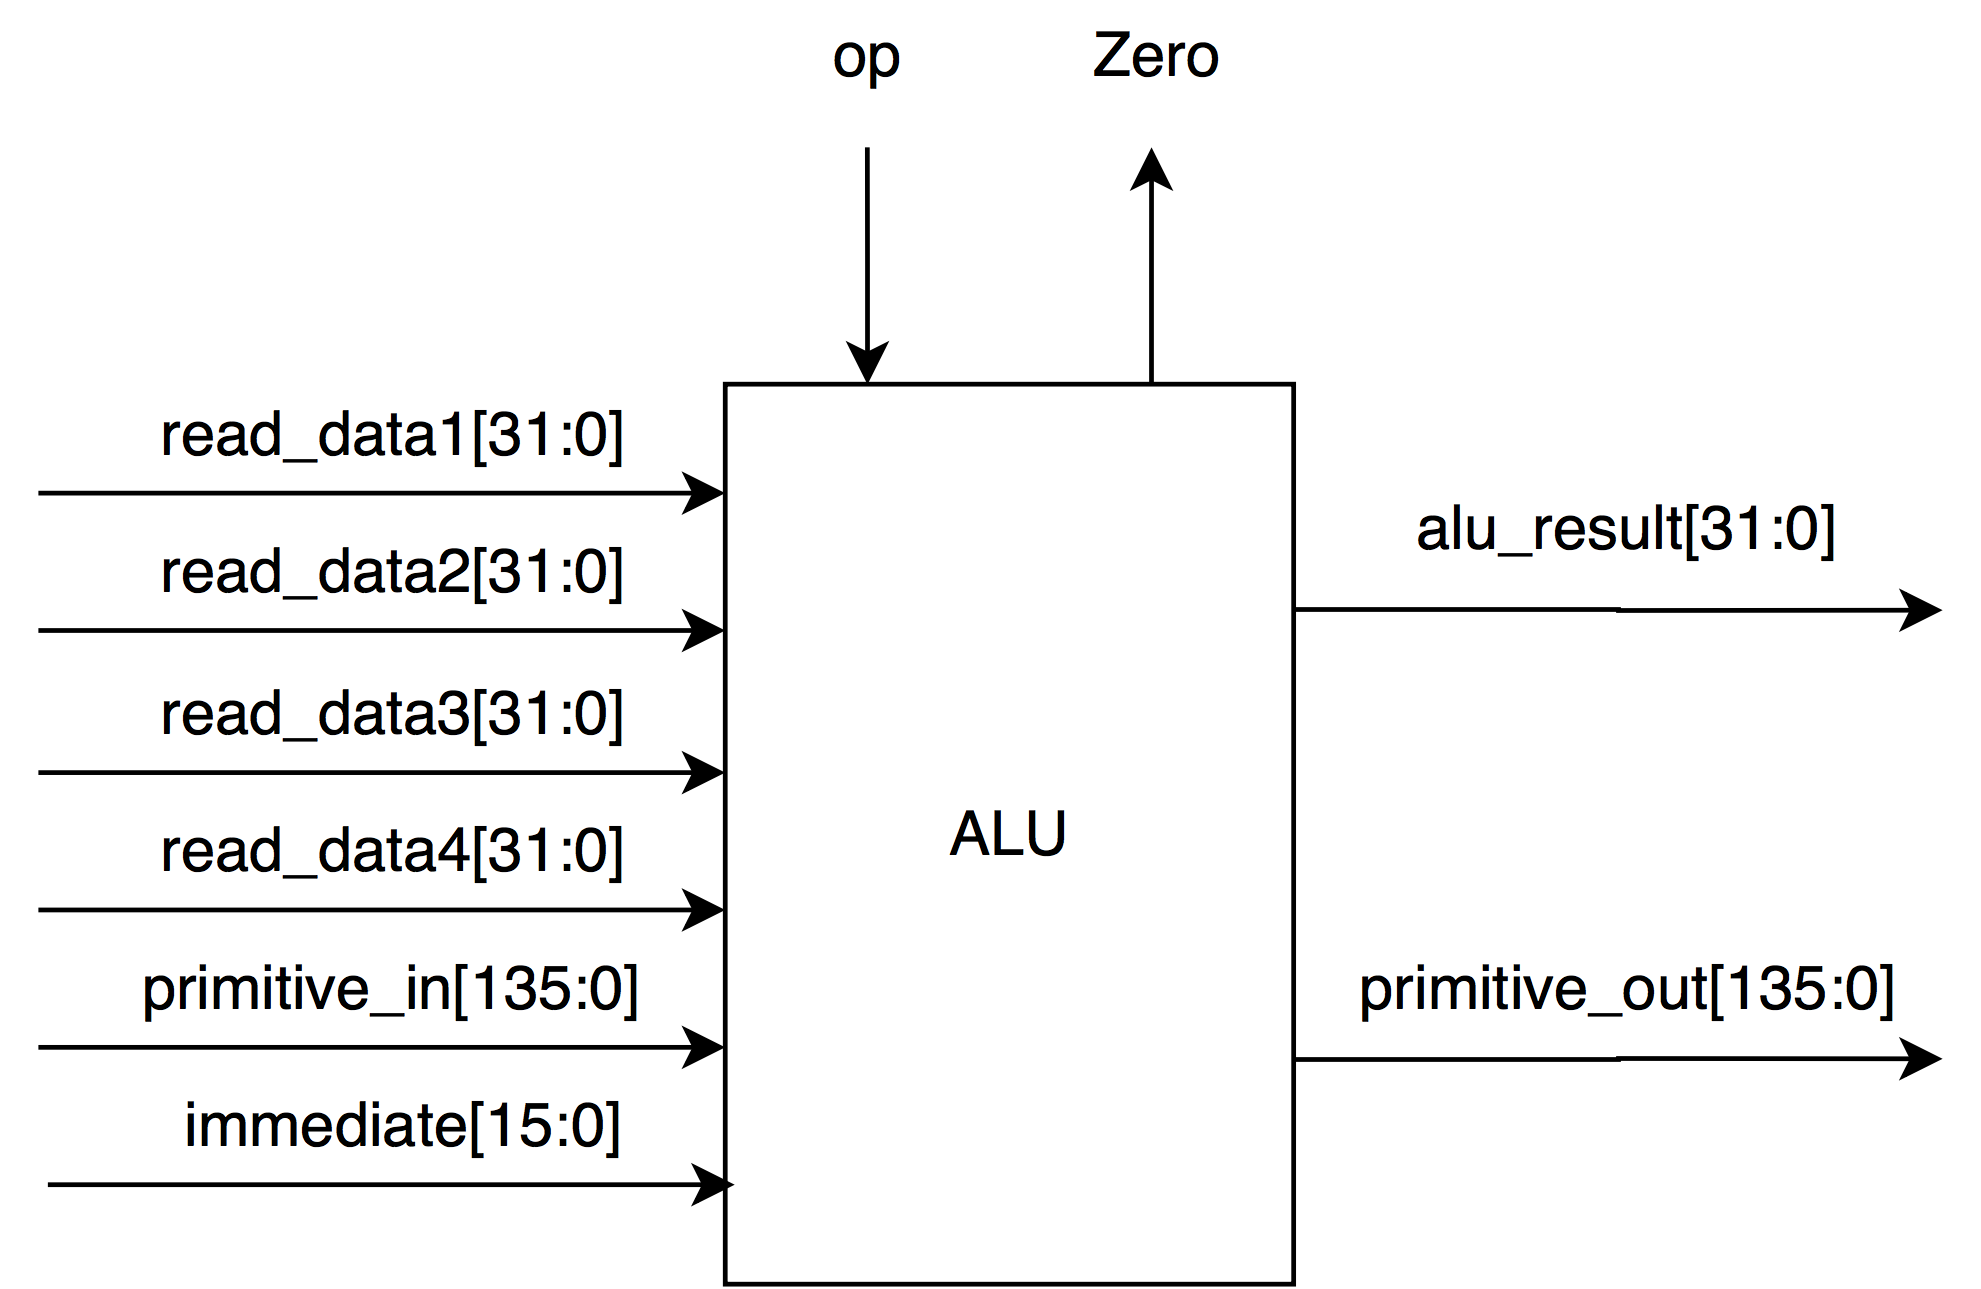
\includegraphics[width=0.8\linewidth]{images/ALU.png}
    \caption{I/O for the ALU.}
    \label{fig:ALU}
\end{figure}

The ALU is the main functional unit of the processor.
It is responsible for performing arithmetic and logical operations on operands from the registers.
Additionally, it supports a number of operations associated with vector primitives.
For the initialization instructions, \texttt{line}, \texttt{bezquad} and \texttt{bezcube}, coordinates read from the general purpose registers are assembled into primitives.
\texttt{getp\{1,2,3,4\}} and \texttt{setp\{1,2,3,4\}} work on individual parts of a primitive.

As shown in Figure \ref{fig:ALU}, the unit also receives an immediate value, taken straight from the decoded instruction, and a control signal, \texttt{op}, which determines the operation to be performed.

\subsection{Data and Scene Memories}

Scene and data memories have similar interfaces, see Figure \ref{fig:data-scene-memories}, the major exception being data width and size.
Data words in scene memory are 136 bits wide, with space for 1024 words.
To allow for the rather unusual word size as well as allowing both the processor core and the output module to interface with the scene memory simultaneously, the scene memory was instantiated as a block RAM on the FPGA.
Words in general data memory are 32 bits wide.
Their input address bus determines either which address to read from or write to.
The \texttt{write\_enable} control signal specifies whether a read or write should be performed.

\begin{figure}[h!]
    \centering
    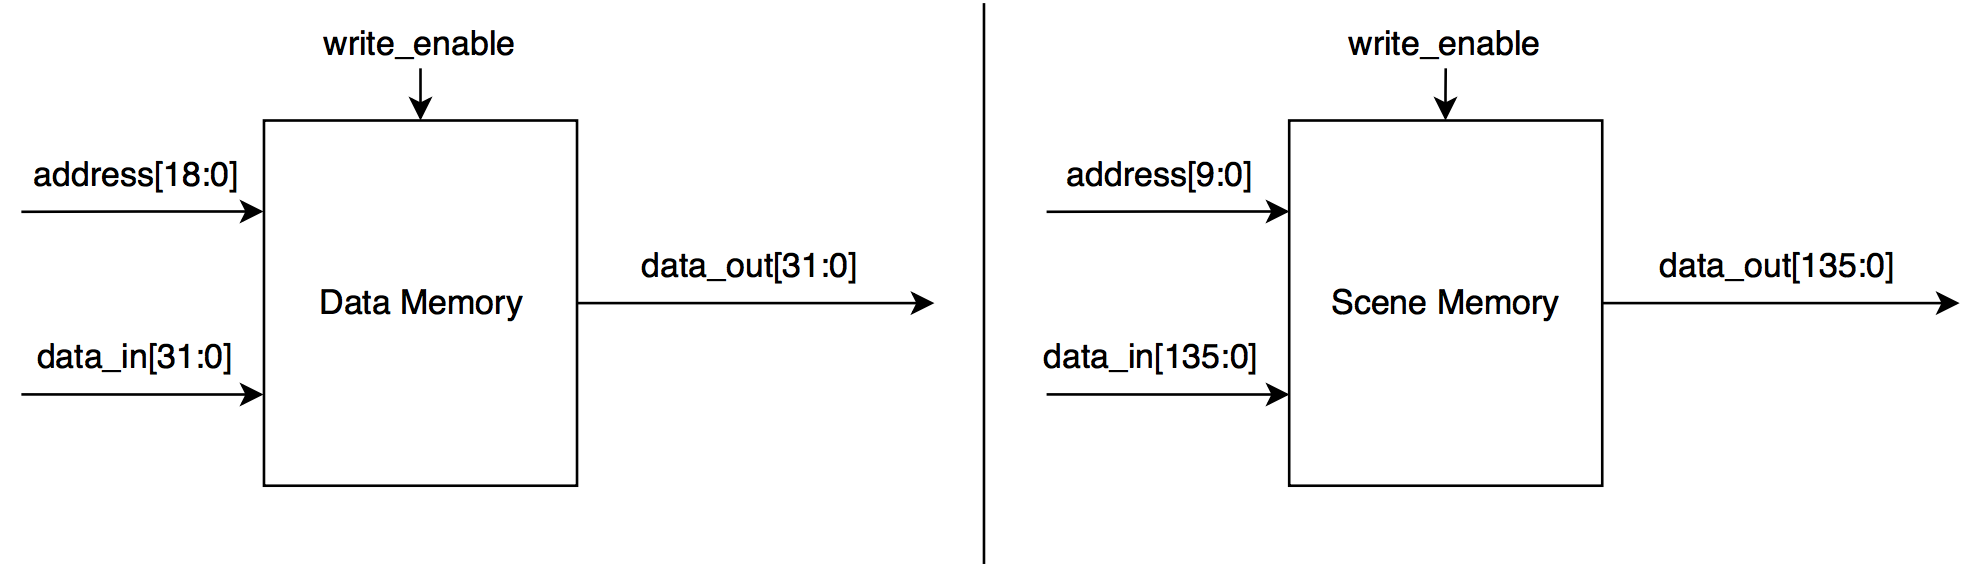
\includegraphics[width=0.9\linewidth]{images/data-scene-memories.png}
    \caption{I/O for data and scene memory modules.}
    \label{fig:data-scene-memories}
\end{figure}


\section{Control Path}

Having examined how instruction, data words and primitives move through the system, this section elaborates on the how the various components involved in the data path are controlled, and what determines their behavior.

Every time a new instruction is read, it is decoded and relevant parts fed into a control unit.
Depending on the instruction, the unit sets its output control signals so that the modules they control behave as desired.
Figure \ref{fig:controlpath} shows how control signals are routed.
Table \ref{tbl:control-signals} lists all control signals and their functionalities.

The control unit maintains processor state.
Since the prototype implemented by the group is non-pipelined, a simple state machine with three states is sufficient.
These are fetch, execute and stall.
Figure \ref{fig:state-machine} shows the states and the conditions for transitioning between them.

While an instruction is being read, the processor is in the fetch state.
To avoid modifying data in registers or in memory, control signals are set to values that disable any writing operations.
In the execute state, control signals are determined by the instruction.
In the case of a stall, the control signals are maintained until the word to be loaded has been written into its destination.

The final functionality implemented in the control unit is a primitive counter.
All instructions that either add new or remove existing instructions in the scene memory cause the counter to be incremented or decremented respecively.
This signal is used in the output module.

\begin{figure}[h!]
    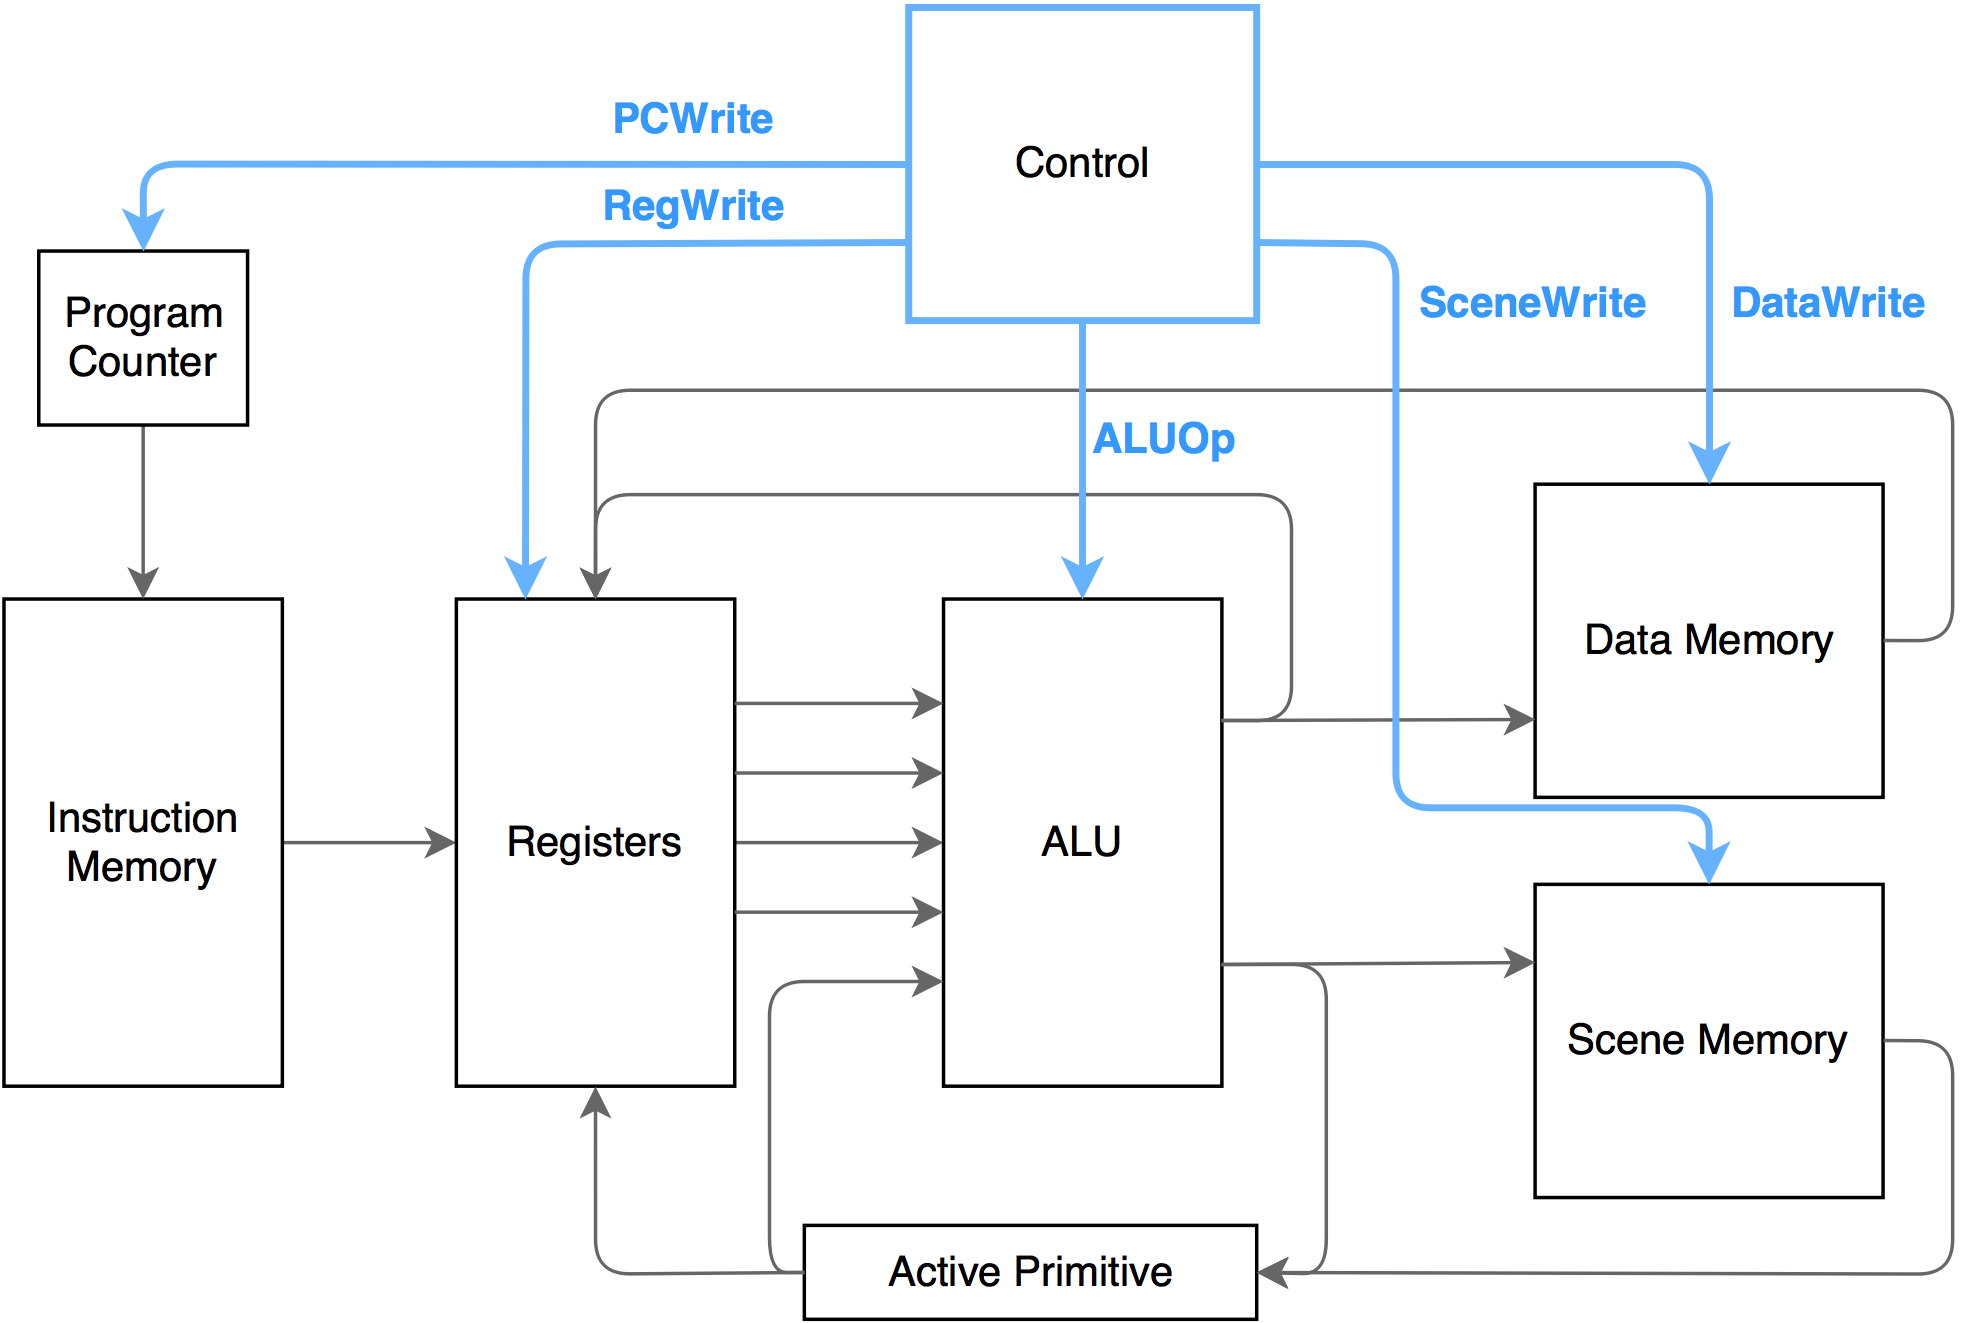
\includegraphics[width=\linewidth]{images/Control_signals.png}
    \caption{RTL sketch of the control path.}
    \label{fig:controlpath}
\end{figure}

\begin{figure}[h!]
    \centering
    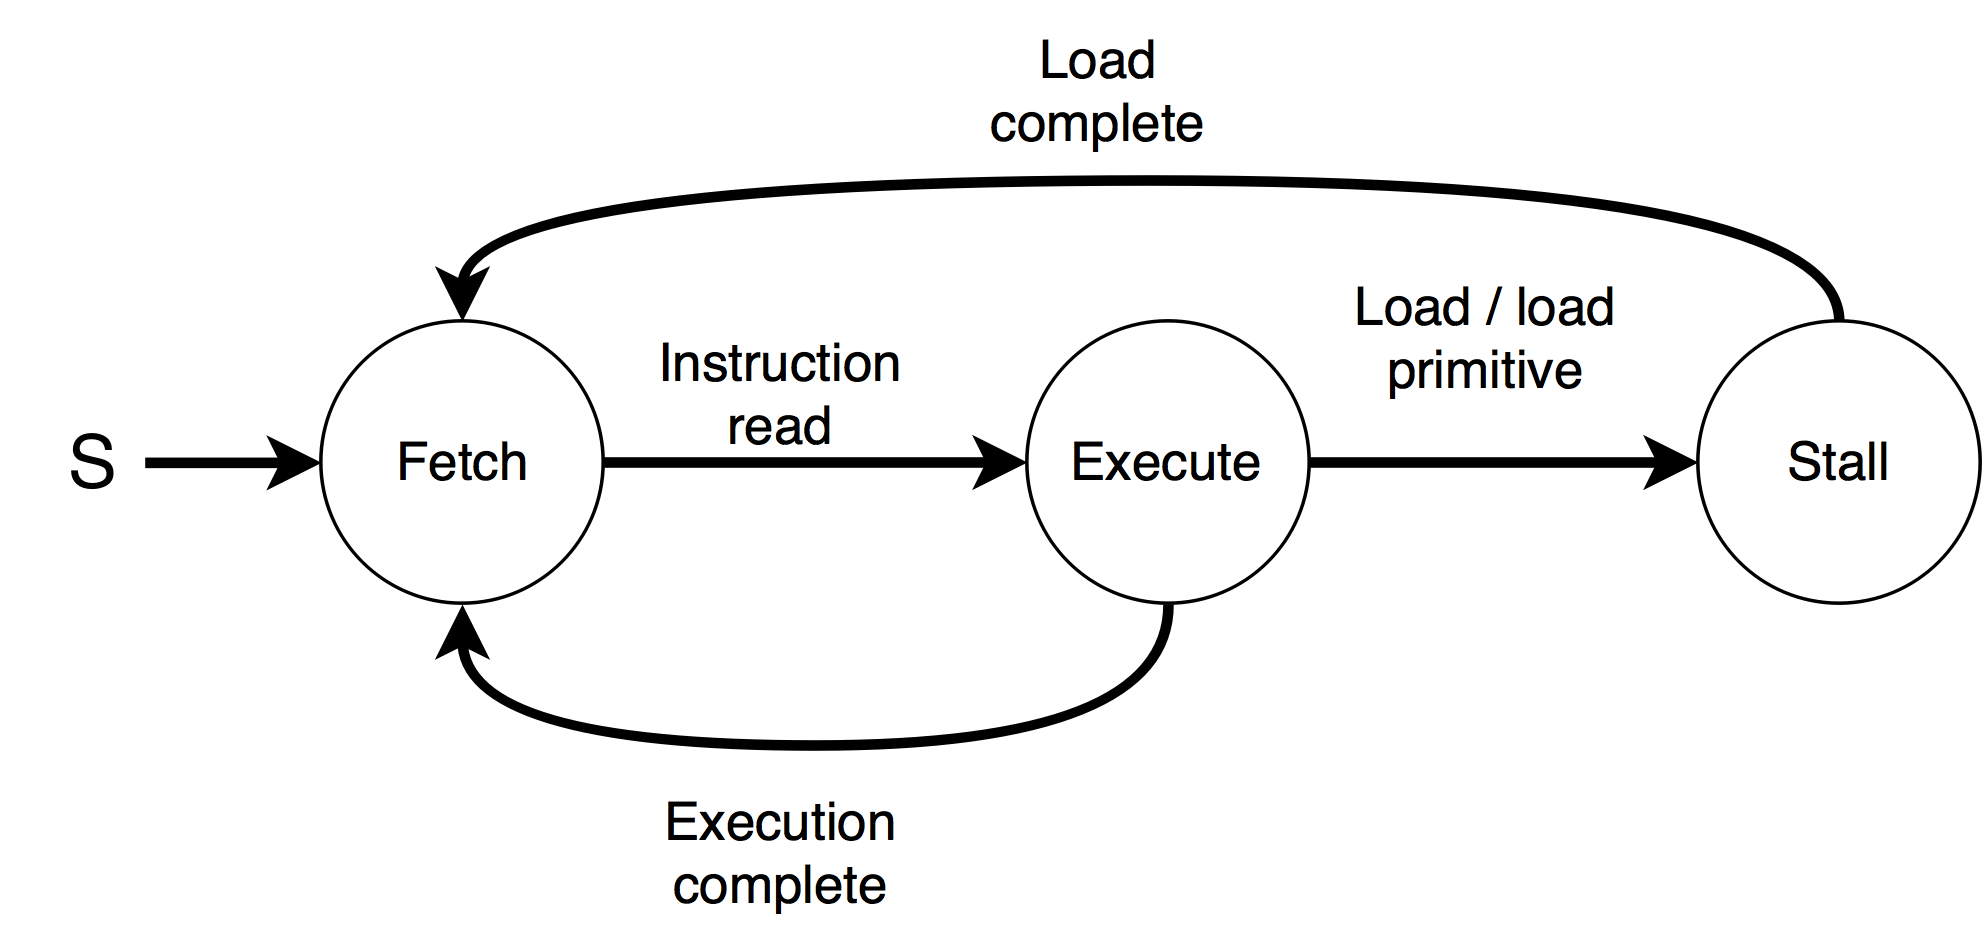
\includegraphics[width=0.7\linewidth]{images/state-machine.png}
    \caption{Processor core state machine.}
    \label{fig:state-machine}
\end{figure}

\begin{table}
    \centering
    \begin{tabular}{|p{5cm}|p{7cm}|}
        \hline
        Signal             & Description                                                                                                                 \\ \hline
        \texttt{reg\_dest}          & Signalizes which register register address from the instruction to use as a destination register.                           \\ \hline
        \texttt{reg\_write}         & Boolean indicator for wether or not to write to the register file.                                                          \\ \hline
        \texttt{prim\_reg\_write}   & Boolean indicator for wether or not to write to the primitive register.                                                     \\ \hline
        \texttt{mem\_to\_reg}       & Determines wether the result from the ALU or a word read from data memory should be used when writing to the register file. \\ \hline
        \texttt{prim\_mem\_to\_reg} & Determines which value should be used to overwrite the primitive register, from the ALU or from the scene memory.           \\ \hline
        \texttt{mem\_write}         & Write enable for the data memory.                                                                                           \\ \hline
        \texttt{prim\_mem\_write}   & Write enable for the scene memory.                                                                                          \\ \hline
        \texttt{branch}             & Indicates that the current instruction is a branch instruction.                                                             \\ \hline
        \texttt{jump}               & Indicates that the current instruction is a jump instruction.                                                               \\ \hline
    \end{tabular}
    \caption{An overview of control signals and their function.}
    \label{tbl:control-signals}
\end{table}
